% O projeto é construído a partir do modelo padrão de livro do LaTeX. As 
% diretrizes da UFMG requerem que o tamanho da fonte seja 12 pontos, a folha 
% seja do tamanho A4 e que tenha só uma coluna de texto.
\documentclass[12pt,a4paper,oneside]{book}

% Suporte a caracteres da língua portuguesa. Se você estiver escrevendo em 
% inglês, remova essa linha.
\usepackage[brazil]{babel} 

% Inclui a lista de pacotes utilizados. Você pode adicionar novos pacotes aqui 
% ou dentro do arquivo pacotes.tex.
\usepackage[utf8]{inputenc} % Suporte a caracteres UTF-8
\usepackage{mathptmx} % Fonte Times New Roman (aproximada)
\usepackage{setspace} % Controle de espaçamento entre linhas
\usepackage{parskip} % Configuração de parágrafos (sem indentação e com espaço entre parágrafos)
\usepackage{indentfirst} % Indenta o primeiro parágrafo de cada seção
\usepackage{geometry} % Configuração das margens
\usepackage{titling} % Configurações de título e autor
\usepackage{emptypage} % Remove números e cabeçalhos de páginas vazias
\usepackage{ragged2e} % Alinhamento justificado à esquerda e à direita
\usepackage[table,xcdraw]{xcolor} % Suporte a cores em tabelas e desenhos
\usepackage{graphicx} % Inclusão de gráficos e imagens
\usepackage[algoruled, portuguese, linesnumbered]{algorithm2e} % Algoritmos com numeração de linhas e estilo específico
\usepackage[hidelinks]{hyperref} % Hiperlinks sem molduras coloridas
\usepackage[round,colon,sort]{natbib} % Citações bibliográficas com estilo específico
\usepackage[nottoc,notlot,notlof]{tocbibind} % Inclui "Referências" no índice
\usepackage{amsmath, amssymb, amsfonts, amsthm, mathtools} % Pacotes AMS para matemática avançada
\usepackage{enumitem} % Personalização de listas enumeradas
\usepackage{bm} % Fonte negrito para símbolos matemáticos
\usepackage{subfig} % Subfiguras dentro de figuras
\usepackage{float} % Controle preciso de posicionamento de figuras e tabelas
\usepackage{mathrsfs} % Fonte para matemática
\usepackage{lscape} % Páginas em modo paisagem
\usepackage{booktabs} % Linhas de qualidade superior para tabelas
\usepackage{csvsimple} % Importação de dados CSV
\usepackage{pdfpages} % Inclusão de páginas PDF
\usepackage{multirow} % Células de múltiplas linhas em tabelas
\usepackage{icomma} % Uso de vírgulas em expressões matemáticas
\usepackage{listings} % Inclusão de códigos fonte
\usepackage[font=itshape]{quoting} % Citações com formatação específica
\usepackage{makecell} % Personalização de células em tabelas
\usepackage{fancyhdr} % Configurações avançadas de cabeçalhos e rodapés
\usepackage{blindtext} % Texto de exemplo


% Inclui as configurações do documento. Você pode adicionar novas configurações
% aqui ou dentro do arquivo configuracoes.tex.
% Este é um arquivo para ajuste de configurações do documento. Aqui você pode definir as configurações de pacotes, comandos personalizados, estilos de página, etc.

% Configuração de cabeçalhos e rodapés
\pagestyle{fancy}
\fancyhf{} % Limpa todos os cabeçalhos e rodapés predefinidos
\fancyhead[R]{\thepage} % Número da página no cabeçalho direito
\fancypagestyle{plain}{%
    \fancyhf{}%
    \fancyhead[R]{\thepage}%
}
\renewcommand{\headrulewidth}{0pt} % Remove a linha horizontal do cabeçalho em todos os estilos

\onehalfspacing % Define o espaçamento entre linhas para 1,5
\geometry{left=3cm, top=3cm, bottom=2cm, right=2cm} % Define as margens do documento: esquerda 3 cm, topo 3 cm, inferior 2 cm, direita 2 cm
\setlength{\parindent}{1.25cm} % Define a indentação do parágrafo para 1,25 cm
\setlength{\parskip}{0cm} % Define o espaçamento entre parágrafos para 0 cm
\renewcommand\contentsname{Sumário} % Renomeia o título do sumário para "Sumário"

% Define novos ambientes para teoremas, lemas, proposições, corolários, resultados e definições. Você deve traduzir para o inglês se estiver escrevendo em inglês.
\newtheorem{theorem}{Teorema} % Define o ambiente "theorem" com a numeração independente
\newtheorem{lemma}[theorem]{Lema} % Define o ambiente "lemma" com a mesma numeração do ambiente "theorem"
\newtheorem{proposition}[theorem]{Proposição} % Define o ambiente "proposition" com a mesma numeração do ambiente "theorem"
\newtheorem{corollary}[theorem]{Corolário} % Define o ambiente "corollary" com a mesma numeração do ambiente "theorem"
\newtheorem{result}[theorem]{Resultado} % Define o ambiente "result" com a mesma numeração do ambiente "theorem"
\newtheorem{definition}[theorem]{Definição} % Define o ambiente "definition" com a mesma numeração do ambiente "theorem"

% Definir o comando para armazenar o subtítulo
\newcommand{\thesubtitle}{}
\newcommand{\subtitle}[1]{\renewcommand{\thesubtitle}{#1}}

% Exemplo de comando personalizado
\newcommand{\brho}{\boldsymbol{\rho}}
\newcommand{\brhop}{\boldsymbol{\rho^\prime}}

% Define o título e autor do trabalho. Você pode alterar esses valores aqui.
\title{Título do Trabalho}

% Caso houver, você DEVE descomentar as correspondentes linhas de código nos 
% arquivos folhaderosto.tex e capa.tex.
% \subtitle{Subtítulo do Trabalho} 

% Define o nome da pessoa autora. Você pode alterar esse valor aqui.
\author{Nome da pessoa autora}

\begin{document}

    % Desativa numeração de páginas nos primeiros elementos do documento.
    \pagenumbering{gobble}

    % Capa
    % Cria a capa do trabalho. Para trabalhos em inglês, é só reescrever a unidade (ex: School of Engineering) e o programa (ex: Graduate Program in Electrical Engineering).

\begin{titlepage}

    \begin{center}
        \begin{spacing}{1}
            UNIVERSIDADE FEDERAL DE MINAS GERAIS \\
            Escola de Engenharia \\
            Colegiado do Curso de Graduação em Engenharia ... \\ % Ou Programada de Pós-Graduação em Engenharia ...
        \end{spacing}
        \vspace{5cm}
        \theauthor \\
        \vspace{5cm}
        \textbf{\MakeUppercase\thetitle}\\ % Caso não tenha subtítulo.
        % \textbf{\MakeUppercase\thetitle: \MakeLowercase\thesubtitle}\\
        \vspace*{\fill}
        Belo Horizonte\\2023
    \end{center}

\end{titlepage}

    % Folha de rosto
    % Folha de Rosto

\newpage
\thispagestyle{empty}
\begin{center}
    \theauthor\\
    \vspace{5cm}
    \textbf{\MakeUppercase\thetitle} % Caso não tenha subtítulo.
    % \textbf{\MakeUppercase\thetitle: \MakeLowercase\thesubtitle}
\end{center}
\vspace{5cm}
\hfill
\begin{minipage}{8cm}
    Trabalho de Conclusão de Curso apresentado ao Curso de Engenharia de Sistemas da Universidade Federal Minas Gerais, como requisito parcial para o grau de bacharel (a) em Engenharia de Sistemas.\\[3mm]
    % Dissertação apresentada ao Programa de Pós-Graduação em Engenharia Elétrica da Universidade Federal de Minas Gerais como requisito parcial para obtenção do título de Mestre em Engenharia Elétrica.\\[3mm]
    % Tese apresentada ao Programa de Pós-Graduação em Engenharia Elétrica da Universidade Federal de Minas Gerais como requisito parcial para obtenção do título de Doutor em Engenharia Elétrica.\\[3mm]
    % Thesis presented to the Graduate Program in Electrical Engineering at the Federal University of Minas Gerais as a partial requirement to obtain the title of Doctor in Electrical Engineering.\\[3mm]
    Orientadora: Profa. Dra. Fulana Beltrano \\[3mm] % Inglês: Supervisor
    Coorientador: Prof. Dr. Ciclano da Silva % Inglês: Co-supervisor	
\end{minipage}\\
\begin{center}
    \vspace*{\fill}
    Belo Horizonte\\2024
\end{center}

    % Ficha catalográfica: só para trabalhos de mestrado e doutorado.
    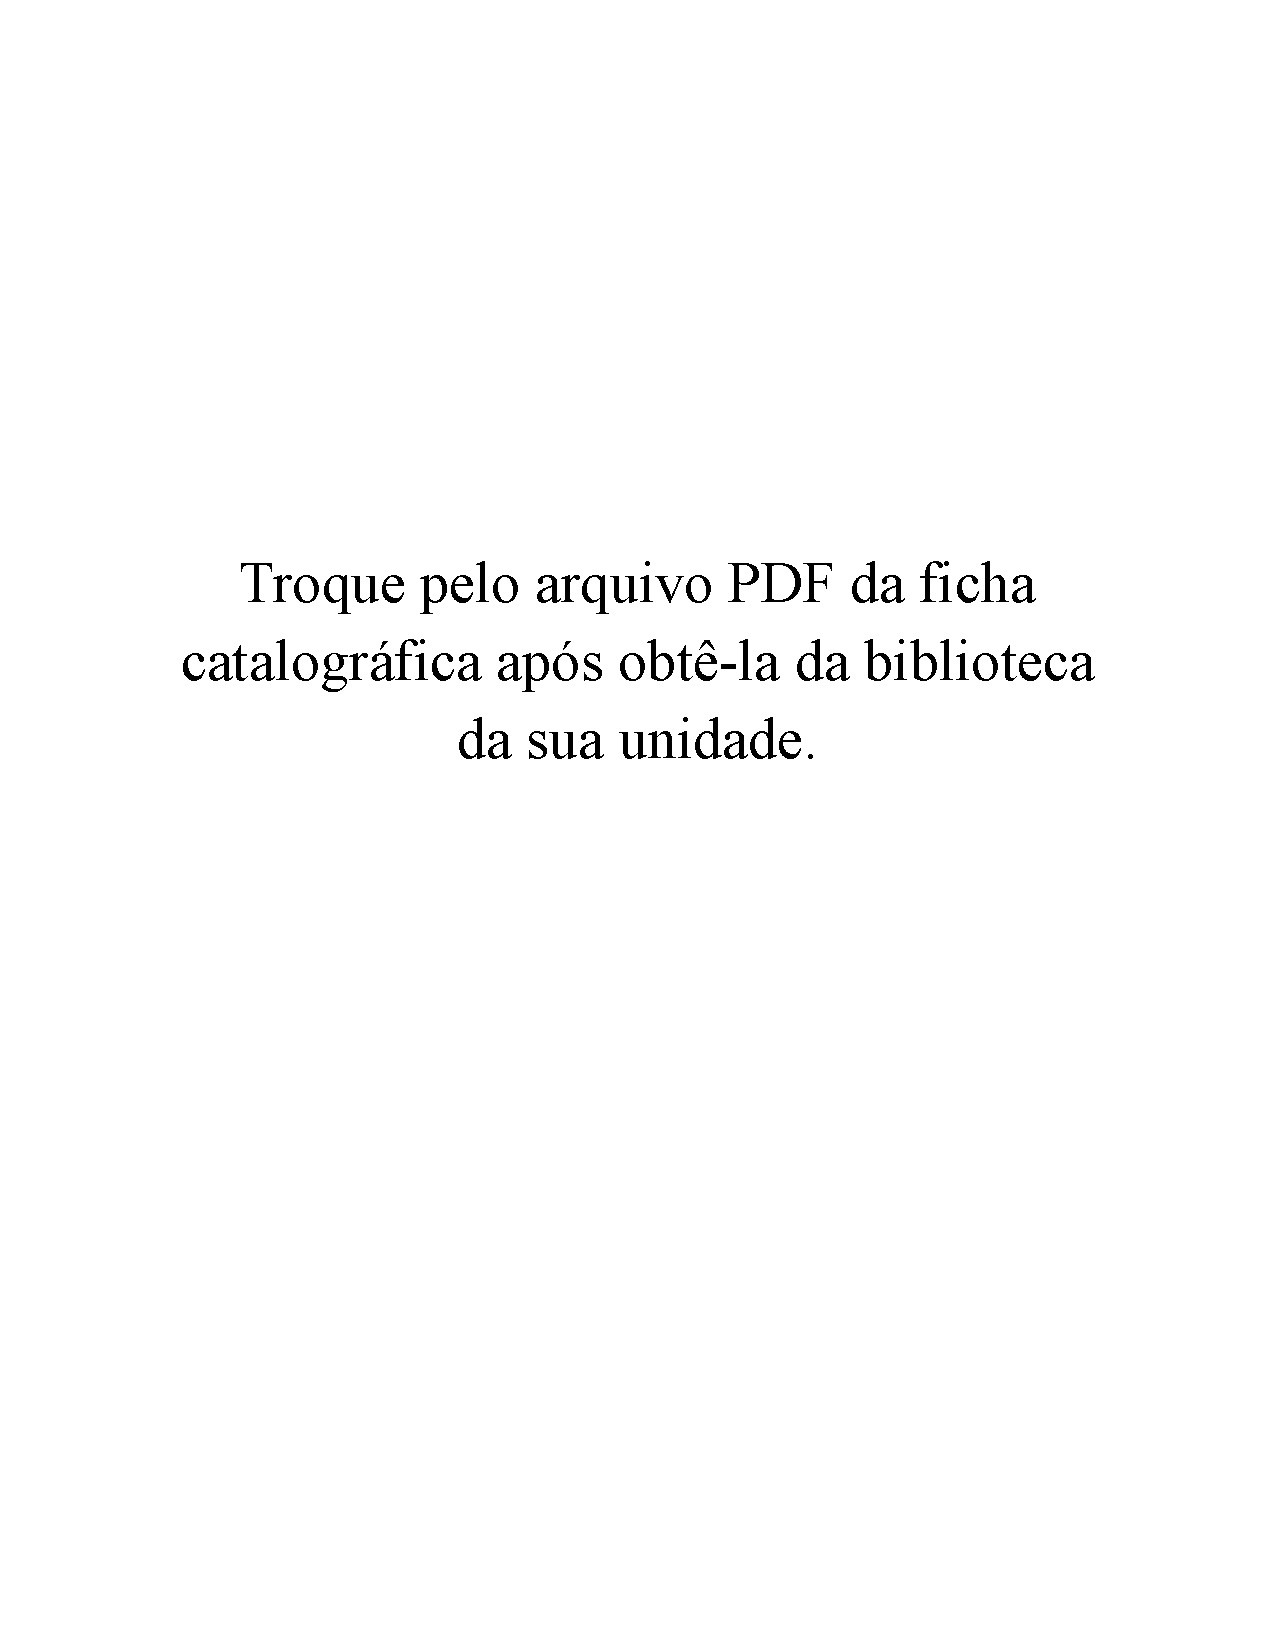
\includepdf{./pretextuais/fichacatalografica}

    % Folha de Aprovação/Ata de defesa: só para trabalhos de mestrado e 
    % doutorado. Caso a ata tenha 2 páginas, você alterar o parâmetro pages={1}
    % para pages={1-2}.	
    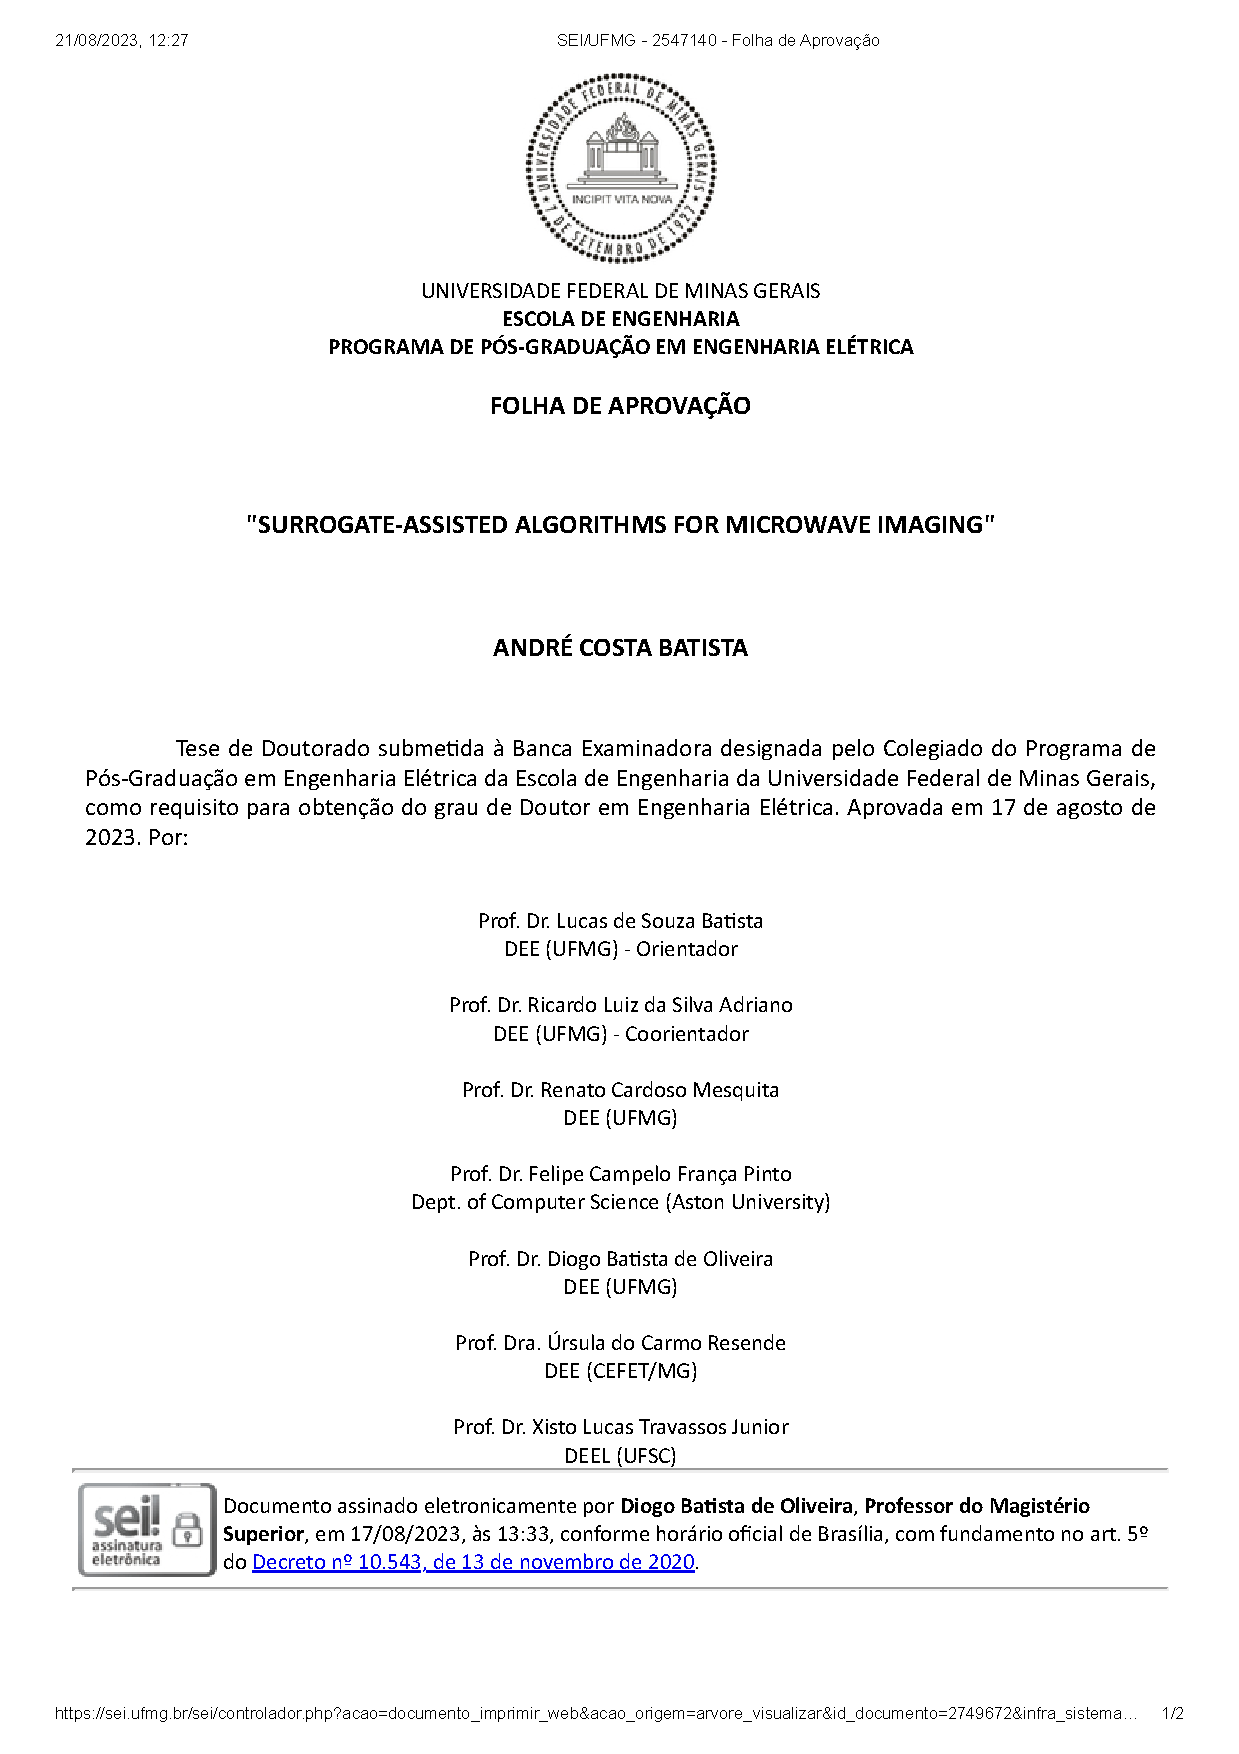
\includepdf[pages={1}]{./pretextuais/folhaaprovacao}

    % Dedicatória
    % A dedicatória, elemento opcional, é utilizada pelo autor para homenagear
% pessoa(s) a quem se dedica o trabalho. O texto é breve, apresentado ao final 
% da página com recuo de 8 cm à esquerda e a página não apresenta título.

\newpage
\thispagestyle{empty}
\vspace*{\fill}
\begin{flushright}
	\hspace{8cm}\textit{Esse trabalho é dedicado à aquela pessoa.}
\end{flushright}

    % Agradecimentos
	% s agradecimentos são destinados à menção de pessoas e instituições que 
% tenham contribuído para o desenvolvimento do trabalho.

\newpage

\chapter*{Agradecimentos} % Inglês: Acknowledgements

	Você pode escrever aqui os agradecimentos a pessoas que contribuíram para a realização do trabalho.
	
	\thispagestyle{empty}

    % Epígrafe
    % As epígrafes são empregadas quando o autor deseja apresentar uma citação 
% direta que estabelece relação com o trabalho apresentado. A página em que 
% consta, não apresenta título “Epígrafe”. Este recurso pode ser utilizado, 
% também, na abertura de cada uma das seções primárias do texto. 

\newpage
\thispagestyle{empty}
\vspace*{\fill}
\begin{flushright}
	``Aqui vai uma bela e inspiradora frase.''
\end{flushright}

    % Resumo e Abstract
	\chapter*{Resumo}

	\noindent O Imageamento em Microondas é uma importante técnica de teste e avaliação não-destrutiva e não-invasiva com muitas aplicações em diversas áreas, como em exames médicos, triagem de segurança, sensoriamento remoto, entre outras. A técnica é baseada em um Problema Inverso de Espalhamento Eletromagnético onde as propriedades elétricas de um meio são recuperadas através de medições de campo espalhado. Além de ser um problema mal-posto, também é não-linear e multimodal. Existem vários métodos numéricos para resolver o problema e eles podem ser classificados em qualitativos ou quantitativos. Estes últimos também são classificados em métodos determinísticos ou estocásticos. Esta tese apresenta uma nova abordagem quantitativa determinística para imageamento em microondas usando algoritmos assistidos por modelos substitutos. O objetivo é abordar os desafios do problema inverso considerando a imagem qualitativa recuperada pelo Método de Amostragem de Ortogonalidade e transformando a imagem em um problema de otimização bidimensional. O método proposto se concentra em otimizar a estimativa de contraste e a operação de limiarização para minimizar o erro da equação de dados. A tese apresenta três formulações baseadas em Algoritmos Evolutivos e duas baseadas em Métodos de Direções de Busca, fornecendo um leque de opções para a resolução do problema de otimização. Além disso, uma nova estrutura é proposta para o desenvolvimento e teste de algoritmos para o problema. A estrutura inclui um pacote abrangente chamado \textit{eispy2d}, que oferece funcionalidades como geração de conjuntos de teste com controle de parâmetros, uma coleção de indicadores de desempenho (incluindo dois novos indicadores) e suporte para comparação estatística de diferentes algoritmos. Os resultados dos experimentos demonstram a eficácia dos métodos propostos. Em cenários com espalhadores fracos, os métodos propostos foram capazes de reconstruir imagens comparáveis àquelas obtidas por métodos tradicionais, enquanto alcançavam tempos de execução próximos. Além disso, em cenários mais desafiadores onde os métodos tradicionais falharam, os algoritmos propostos mostraram resultados consistentes em termos de recuperação de imagens.

	\vspace{5mm}
	
	\noindent\textbf{Palavras-chaves}: imageamento em microondas; problemas inversos; algoritmos assistidos por modelos substitutos; algoritmos evolutivos; métodos de direção de busca; biblioteca de código aberto.
	
	\thispagestyle{empty}
    \chapter*{Abstract}

	\noindent Microwave Imaging is an important nondestructive and noninvasive testing and evaluating technique with many applications in diverse areas, such as medical imaging, security screening, remote sensing, among others. The technique is based on an Electromagnetic Inverse Scattering Problem where the electric properties of a medium are recovered through scattered field measurements. Besides being an ill-posed problem, it is also nonlinear and multimodal. There are several numerical methods for solving the problem and they can be classified into qualitative and quantitative ones. The latter is also classified into deterministic and stochastic methods. This thesis presents a novel quantitative deterministic approach for microwave imaging using surrogate model-assisted algorithms. The objective is to address the challenges of the inverse problem by considering the qualitative image recovered by the Orthogonality Sampling Method and transforming it into a two-dimensional optimization problem. The proposed method focuses on optimizing the contrast estimation and the threshold operation to minimize the data equation error. The thesis introduces three formulations based on Evolutionary Algorithms and two ones based on Descent Methods, providing a range of options for solving the optimization problem. In addition, a new framework is proposed for the development and testing of algorithms in microwave imaging. The framework includes a comprehensive package called \textit{eispy2d}, which offers functionalities such as test set generation with parameter control, a collection of performance indicators (including two novel indicators), and support for statistical comparison of different algorithms. The results of the experiments demonstrate the effectiveness of the proposed methods. In weak scatterer scenarios, the surrogate model-assisted algorithms were able to recover images that were comparable to those obtained by traditional methods, while achieving similar runtimes. Moreover, in more challenging scenarios where traditional methods failed, the proposed algorithms showed consistent results in terms of image recovery.
	
	\vspace{5mm}
	
	\noindent\textbf{Keywords}: microwave imaging; inverse problems; surrogate model-assisted algorithms; evolutionary algorithm; descent methods; open-source package.
	
	\thispagestyle{empty}
	

	% Listas
    \begingroup
    \pagestyle{empty}
    \listoffigures
    \pagestyle{empty}
    \listoftables
    \pagestyle{empty}
    \listofalgorithms
\endgroup
	
    % Abreviações e símbolos
	% Siglas e abreviaturas utilizadas no texto devem ser apresentadas em uma lista 
% alfabética seguida de sua grafia por extenso. A primeira vez que a sigla 
% aparece no texto deve-se pontuar a expressão por extenso, seguida da sigla 
% entre parênteses; nas demais vezes, utiliza-se somente a sigla, inserida
% diretamente no texto.

\newpage
\chapter*{Lista de Siglas e Símbolos} % Inglês: List of Abbreviations and Symbols

	\section*{Siglas}
	
		\begin{itemize}[labelwidth=5em,leftmargin=\dimexpr\labelwidth+\labelsep\relax,align=left]
			\item[ACO] Ant Colony Optimization
			\item[BIM] Born Iterative Method
			\item[CNN] Convolutional Neural Networks
			\item[DE] Differential Evolution
			\item[EA] Evolutionary Algorithm
			\item[GA] Genetic Algorithm
			\item[GAN] Generative Adversarial Network
			\item[PSO] Particle Swarm Optimization
			\item[TMz] Modo Magnético Transversal em $z$
		\end{itemize}
	
		\thispagestyle{empty}

	\section*{Símbolos}
	
		\thispagestyle{empty}
	
		\begin{itemize}[labelwidth=4em,leftmargin=\dimexpr\labelwidth+\labelsep\relax,align=left]
			\item[$\epsilon$] Permissividade complexa [F/m + $j\Omega$/m]
			\item[$\epsilon_r$] Permissividade relativa
			\item[$\theta$] Ângulo da coordenada polar [rad]
			\item[$\lambda_b $] Comprimento de onda de fundo [m]
			\item[$\sigma$] Condutividade [$\Omega$/m]
			\item[$\phi$] Ângulo de incidência [rad]
			\item[$\mathbf{E}$] Vetor de intensidade elétrica [V/m]
			\item[$E_z$] Componente $z$ do vetor de intensidade elétrica [V/m]
			\item[$k$] Número de onda [1/m]
			\item[$\mathbb{R}$] Conjunto dos números reais
			\item[$\mathbf{r}$] Vetor posição no espaço 3D [m]
			\item[$x, y, z$] Coordenadas cartesianas [m]
			\item[$V$] Espaço tridimensional
		\end{itemize}
	
		\thispagestyle{empty}
	
	
    
    % Sumário
    \thispagestyle{empty}
    \tableofcontents

    % Ativa numeração de páginas
    % ATENÇÃO: depois que você terminar de escrever o trabalho, você DEVE
    % voltar aqui acertar esse contador. A folha de rosto é a página 1. A partir 
    % disso, você deve fazer a conta para ajustar o contador para o número 
    % da página anterior ao primeiro capítulo. Ou seja, se começando pela folha
    % de rosto, você contar que a primeira página da introdução é a página 10,
    % então você deve ajustar o contador para 9. 
    \pagenumbering{arabic}
    \setcounter{page}{9}

    % Introdução
    % ------------------------------------------------------------------------------
% Introdução
% ------------------------------------------------------------------------------

\chapter{Introdução}\label{chap:introducao} % Inglês: Introduction

	Parte inicial do texto na qual se apresenta a delimitação do assunto tratado, os 
	objetivos da pesquisa e outros elementos necessários para apresentar o tema 
	do trabalho. O texto tem o objetivo de introduzir o leitor ao trabalho e 
	apresentar as informações para uma compreensão geral da proposta
	desenvolvida.

	\section{Objetivos Geral e Específicos}\label{sec:introducao:objetivos}

		Descrever os objetivos geral e específicos do trabalho. O objetivo
		geral devem ser claro e conciso, indicando o propósito do trabalho.
		Os objetivos específicos devem ser apresentados de forma a indicar
		os passos necessários para atingir o objetivo geral. Geralmente, em formato de tópicos.

	\section{Contribuições e Originalidade}\label{sec:introducao:contribuicoes}

		Descrever as contribuições do trabalho, indicando o que o trabalho
		propõe de novo ou diferente em relação ao estado da arte. As contribuições
		devem ser claras e objetivas, indicando o que o trabalho agrega ao conhecimento
		existente.
	
	\section{Organização do Trabalho}\label{sec:introducao:organizacao}

		Descrever a organização do trabalho, indicando o conteúdo de cada capítulo
		e a relação entre eles. A organização do trabalho deve ser clara e
		coerente, de forma a facilitar a compreensão do leitor.


    % Revisão Bibliográfica
    % ------------------------------------------------------------------------------
% Revisão Bibliográfica
% ------------------------------------------------------------------------------

\chapter{Revisão Bibliográfica}\label{chap:revisao}

	Ao redigir uma revisão bibliográfica em trabalhos acadêmicos, é crucial adotar uma abordagem sistemática e crítica. Inicie identificando e selecionando fontes relevantes que abordem diretamente o tema de pesquisa, priorizando publicações acadêmicas revisadas por pares, como artigos de periódicos, livros e conferências. Uma boa prática é organizar a literatura em temas ou escolas de pensamento, facilitando a compreensão do leitor sobre o estado da arte e as lacunas existentes. É importante também avaliar criticamente cada obra, discutindo sua contribuição para o campo, metodologias, resultados e limitações. A revisão deve ser escrita de forma coesa, com transições suaves entre os trabalhos discutidos, e deve terminar destacando como a pesquisa atual se insere e contribui para o conhecimento existente. Citando adequadamente todas as fontes, evita-se o plágio e reconhece-se o trabalho dos pesquisadores originais, além de fornecer ao leitor caminhos para aprofundamento.

    % Metodologia
    % ------------------------------------------------------------------------------
% Metodologia
% ------------------------------------------------------------------------------

\chapter{Metodologia}\label{chap:metodologia}

	Redigir um capítulo sobre metodologia em um trabalho acadêmico é fundamental para demonstrar a validade e a confiabilidade da pesquisa. Este capítulo deve detalhar os procedimentos e técnicas utilizados para coletar e analisar dados, permitindo que outros pesquisadores reproduzam o estudo. Aqui estão os passos essenciais para escrever um capítulo de metodologia eficaz:

	\begin{itemize}
		\item Introdução à Metodologia: Comece com uma breve introdução que esclareça o propósito do capítulo e como ele contribui para os objetivos gerais da pesquisa.
		\item Descrição da Pesquisa: Especifique o tipo de pesquisa realizada (qualitativa, quantitativa, mista) e justifique a escolha. Explique como essa abordagem é adequada para responder às perguntas de pesquisa ou hipóteses.
		\item Participantes ou Dados: Descreva a população-alvo, critérios de inclusão e exclusão, e como os participantes ou dados foram selecionados. Para pesquisas experimentais, explique como os grupos de controle e experimentais foram formados.
		\item Instrumentos e Materiais: Liste os instrumentos, ferramentas, ou materiais utilizados na coleta de dados, incluindo questionários, entrevistas, software, etc. Descreva como e por que cada instrumento foi escolhido.
		\item Procedimento: Detalhe todos os passos seguidos durante a coleta de dados. Para experimentos, descreva as condições sob as quais foram realizados, incluindo variáveis controladas e não controladas.
		\item Análise de Dados: Explique as técnicas estatísticas, métodos de análise qualitativa, ou modelos utilizados para analisar os dados coletados. Justifique a escolha desses métodos e discuta sua adequação para o tipo de dados coletados.
		\item Validade e Confiabilidade: Discuta as medidas tomadas para garantir a validade e confiabilidade dos resultados. Isso pode incluir a validação de instrumentos, triangulação de dados, ou testes piloto.
		\item Limitações: Reconheça quaisquer limitações metodológicas que possam afetar os resultados ou a interpretação da pesquisa.
		\item Ética: Se aplicável, descreva as considerações éticas relacionadas à pesquisa, incluindo aprovações de comitês de ética, consentimento informado dos participantes, e como a privacidade e a confidencialidade foram mantidas.
		\item Resumo: Conclua o capítulo com um resumo dos pontos-chave, reforçando como a metodologia adotada permite abordar as perguntas de pesquisa ou testar as hipóteses.
	\end{itemize}

	Lembre-se de que a clareza e a precisão são cruciais neste capítulo. O objetivo é fornecer informações suficientes para que outros pesquisadores possam entender como o estudo foi conduzido e, se desejado, replicar a pesquisa.

    % Resultados
    % ------------------------------------------------------------------------------
% Resultados
% ------------------------------------------------------------------------------

\chapter{Resultados}\label{chap:resultados}
	
	Escrever um capítulo de resultados em trabalhos acadêmicos é uma etapa crucial, pois comunica as descobertas da pesquisa. Aqui estão algumas sugestões para estruturar e redigir este capítulo de forma eficaz:

	\begin{itemize}
		\item Introdução Breve: Comece com uma introdução curta que reitere os objetivos da pesquisa e explique o que será apresentado no capítulo.
		
		\item Organização Lógica: Estruture o capítulo de forma lógica, geralmente seguindo a ordem das perguntas de pesquisa ou hipóteses. Isso ajuda os leitores a acompanhar facilmente as descobertas.
		
		\item Apresentação Clara dos Dados: Apresente os resultados de maneira clara e concisa. Use tabelas, gráficos e figuras para ilustrar os dados de forma eficaz, garantindo que cada um seja claramente rotulado e acompanhado de uma legenda explicativa.
		
		\item Descrição dos Resultados: Forneça uma descrição textual dos resultados, destacando as descobertas principais. 
		
		\item Referência aos Objetivos e Hipóteses: Faça referência explícita aos objetivos da pesquisa ou hipóteses ao apresentar os resultados, indicando como cada resultado se relaciona com eles.
		
		\item Precisão e Objetividade: Mantenha a precisão e objetividade ao relatar os resultados. Evite usar linguagem emotiva ou fazer inferências sem suporte dos dados.
		
		\item Tratamento de Dados Negativos ou Inesperados: Se houver resultados negativos ou inesperados, inclua-os e ofereça uma breve descrição. Esses resultados podem ser tão informativos quanto os positivos.
		
		\item Uso de Subseções: Divida o capítulo em subseções, se necessário, para manter a organização e facilitar a leitura. Cada subseção pode abordar diferentes aspectos dos resultados.
		
		\item Consistência com Metodologia: Garanta que a apresentação dos resultados seja consistente com a metodologia descrita anteriormente. Isso inclui o uso dos mesmos termos e definições.
		
		\item Sumário dos Resultados: Conclua o capítulo com um sumário dos principais resultados.
	\end{itemize}

    % Conclusão
    % ------------------------------------------------------------------------------
% Conclusão
% ------------------------------------------------------------------------------

\chapter{Conclusão}\label{chap:conclusao}
	
	Escrever um bom capítulo de conclusão em trabalhos acadêmicos envolve sintetizar os principais achados da pesquisa, refletir sobre o significado desses resultados, e sugerir direções futuras. Aqui estão algumas diretrizes para estruturar este capítulo:

	\begin{itemize}
		\item Resumo dos Principais Achados: Comece recapitulando os principais resultados da pesquisa. Destaque como esses resultados atendem aos objetivos do estudo ou respondem às perguntas de pesquisa.
		
		\item Contextualização: Discuta a importância dos resultados no contexto do campo de estudo. Isso inclui como seus achados se alinham ou divergem de estudos anteriores.
		
		\item Reflexão Crítica: Inclua uma autoavaliação da pesquisa, abordando limitações e como elas podem ter afetado os resultados. Isso demonstra integridade acadêmica e compreensão das nuances da pesquisa.
		
		\item Implicações Práticas e Teóricas: Explique as implicações dos seus resultados para a prática, teoria ou política. Isso mostra a relevância e o valor do seu trabalho.
		
		\item Sugestões para Pesquisas Futuras: Baseando-se nas limitações e nos achados da sua pesquisa, sugira áreas para futuras investigações. Isso ajuda a avançar o campo de estudo.
		
		\item Conclusão Final: Termine com uma conclusão forte que reafirme a contribuição do seu trabalho para o campo de estudo. Isso pode incluir uma declaração poderosa sobre o significado dos seus achados ou uma visão para o futuro da área de pesquisa.
		
		\item Produção Bibliográfica: Se aplicável, liste as publicações geradas a partir da sua pesquisa. Isso pode incluir artigos, apresentações em conferências, ou outros materiais acadêmicos.
	\end{itemize}


    % Referências bibliográficas
    \bibliographystyle{apalike}
    \bibliography{referencias}
    
    % Apêncice
    \appendix
    % ------------------------------------------------------------------------------
% Apêndice
% ------------------------------------------------------------------------------

	\chapter{Como fazer citações}

		Você pode fazer uma citação de diversas formas. Se você quiser fazer uma citação entre parênteses, você pode fazer assim: \citep{milgram1969note}. Se você quiser mencionar o número da página, você pode fazer assim: \citep[p. 10]{deb2002fast}. Agora, se você quiser fazer uma citação onde o autor é parte da sentença, você pode fazer assim: \cite{maxwell1865viii} afirma que... Se você quiser fazer uma citação com mais de um autor, você pode fazer assim: \citep{van2019fantastic,maxwell1865viii}.
	
	\chapter{Como escrever equações}

		Um exemplo básico de equação:
		\begin{equation}
			\boldsymbol{\mathcal{F}}(\mathbf{r}, t) = \mathfrak{Re}\{\mathbf{F}(\mathbf{r})e^{j\omega t}\} \label{eq:2:fourier}
		\end{equation}

		Um exemplo sobre como escrever múltiplas equações e o uso de fonte cursiva nas letras:
		\begin{eqnarray}
			\nabla\times\boldsymbol{\mathcal{E}}(\mathbf{r}, t) &=& - \frac{\partial\boldsymbol{ \mathcal{B}}}{\partial t}(\mathbf{r}, t) \label{eq:2:maxwell:time:1} \\
			\nabla\times\boldsymbol{\mathcal{H}}(\mathbf{r}, t) &=& \frac{\partial\boldsymbol{ \mathcal{D}}}{\partial t}(\mathbf{r}, t) + \boldsymbol{\mathcal{J}}(\mathbf{r}, t) \label{eq:2:maxwell:time:2} \\
			\nabla\cdot\boldsymbol{\mathcal{D}}(\mathbf{r}, t) &=& \rho(\mathbf{r}, t) \label{eq:2:maxwell:time:3} \\
			\nabla\cdot\boldsymbol{\mathcal{B}}(\mathbf{r}, t) &=& 0 \label{eq:2:maxwell:time:4}
		\end{eqnarray}

		Um exemplo de desenvolvimento de equação:
		\begin{eqnarray}
			\nabla\times\mathbf{H}(\mathbf{r}) &=&  j\omega\epsilon_0\epsilon_r\mathbf{E}(\mathbf{r}) + \sigma(\mathbf{r})\mathbf{E}(\mathbf{r})+ \mathbf{J}_i(\mathbf{r}) \label{eq:2:complexmedia:1} \\
			 &=&  j\omega\epsilon_0\left(\epsilon_r(\mathbf{r}) -j\frac{\sigma(\mathbf{r})}{\omega\epsilon_0}\right)\mathbf{E}(\mathbf{r}) +  \mathbf{J}_i(\mathbf{r}) \label{eq:2:complexmedia:2} \\
			&=&  j\omega\epsilon(\mathbf{r})\mathbf{E}(\mathbf{r}) +  \mathbf{J}_i(\mathbf{r}) \label{eq:2:complexmedia:3}
		\end{eqnarray}

		Um exemplo de equação quebrada em mais de uma linha:
		\begin{multline}
			\chi(\brho)E_{z_i}(\brho) = J_{z_{eq}}(\brho) + \frac{jk_b^2}{4} \chi(\brho) \int_S dS^\prime J_0(k_b|\brho-\brhop|) J_{z_{eq}}(\brhop) \\ + \frac{jk_b^2}{4} \chi(\brho) \int_S dS^\prime Y_0(k_b|\brho-\brhop|) J_{z_{eq}}(\brhop)  \label{eq:2:2d:greendecomp:csie}
		\end{multline}

		Um exemplo de equação com somatórios e integrais:
		\begin{multline}
			\iint_D E_{z_s}(\theta,\phi) w^{(\theta)}_u(\theta) w^{(\phi)}_v(\phi) d\theta d\phi = \\ -\frac{jk_b^2}{4} \sum\limits_{i=1}^{N_I}\sum\limits_{j=1}^{N_J} \sum\limits_{p=1}^{N_P}\sum\limits_{q=1}^{N_Q}\sum\limits_{r=1}^{N_R} a_{ij} b_{pqr} \iint\limits_{D} \iint\limits_{S} d\theta d\phi dxdy~ \bigg[ G^D_{2D}(\theta,x,y) \\ f^{(x)}_i(x) f^{(y)}_j(y) g^{(x)}_{p}(x) g^{(y)}_{q}(y) g^{(\phi)}_r(\phi)w^{(\theta)}_u(\theta) w^{(\phi)}_v(\phi)  \bigg], \\ u = 1,\cdots, N_U,~ v = 1,\cdots,N_V \label{eq:3:discretization:6}
		\end{multline}

		Um exemplo de definição de matriz:
		\begin{equation}
			\boldsymbol{\bar{\Lambda}} = \begin{bmatrix}
																\Lambda_{11} & \Lambda_{12} & \cdots & \Lambda_{1N_V} \\
															   \Lambda_{21} & \Lambda_{22} & \cdots & \Lambda_{2N_V} \\
															   \vdots & \vdots & \vdots & \vdots \\
															   \Lambda_{u1} & \Lambda_{u2} & \cdots & \Lambda_{uN_V} \\
															   \vdots & \vdots & \vdots & \vdots \\
															   \Lambda_{N_U1} & \Lambda_{N_U2} & \cdots & \Lambda_{N_UN_V}
															  \end{bmatrix} \label{eq:discretization:9}
	   \end{equation}

	   Um exemplo de definição de casos:
	   \begin{equation}
		w_{uv} = \begin{cases}
						  1,& \mathrm{in} ~D_{uv}, \\
						  0,& \mathrm{outside}, ~D_{uv}
					  \end{cases} \label{eq:3:discretization:subdomain}
		\end{equation}

		Um exemplo para organização de três matrizes em uma mesma linha:
		\begin{align}
			\boldsymbol{\bar{\chi}} &=	\begin{bmatrix}
														 \chi_{11} & 0 & \cdots & 0 \\
														 0 & \chi_{12} & \cdots & 0 \\
														 \vdots & \vdots & \ddots & \vdots \\
														  0 & 0 & \cdots & \chi_{N_IN_J}
													 \end{bmatrix}
			&\boldsymbol{\bar{\beta}} &=	\begin{bmatrix}
																\beta_{11} & 0 & \cdots & 0 \\
																0 & \beta_{12} & \cdots & 0 \\
																\vdots & \vdots & \ddots & \vdots \\
																0 & 0 & \cdots & \beta_{N_IN_J}
															\end{bmatrix}
			&\mathbf{\bar{R}} &=	\begin{bmatrix}
													R_{11} & 0 & \cdots & 0 \\
													0 & R_{12} & \cdots & 0 \\
													\vdots & \vdots & \ddots & \vdots \\
													0 & 0 & \cdots & R_{N_IN_J}
												\end{bmatrix} \label{eq:3:discretization:collocation:18}
		\end{align}

		Note que você pode referenciar equações das seguintes formas:
		\begin{itemize}
			\item Quando ela estiver no meio da frase, você pode usar simplesmente o comando \verb|\eqref{}|. Por exemplo: ``...como mostrado em \eqref{eq:2:maxwell:time:1}, ...''
			\item Quando você estiver no início da frase, você pode escrever: ``A Eq. \eqref{eq:2:maxwell:time:1} mostra que...''
		\end{itemize}
	
	\chapter{Como inserir figuras}

		Um exemplo sobre como inserir figuras simples pode ser visto em \ref{fig:2:scattering}. Você pode referenciar figuras através do comando \verb|\ref{}| ou do comando \verb|\autoref{}|. O primeiro comando apenas referencia o número da figura, enquanto o segundo comando referencia o número da figura e o nome dela. Por exemplo, você pode escrever: ``...como mostrado na \autoref{fig:2:scattering}, ...''.
		\begin{figure}[!tb]
			\centering
			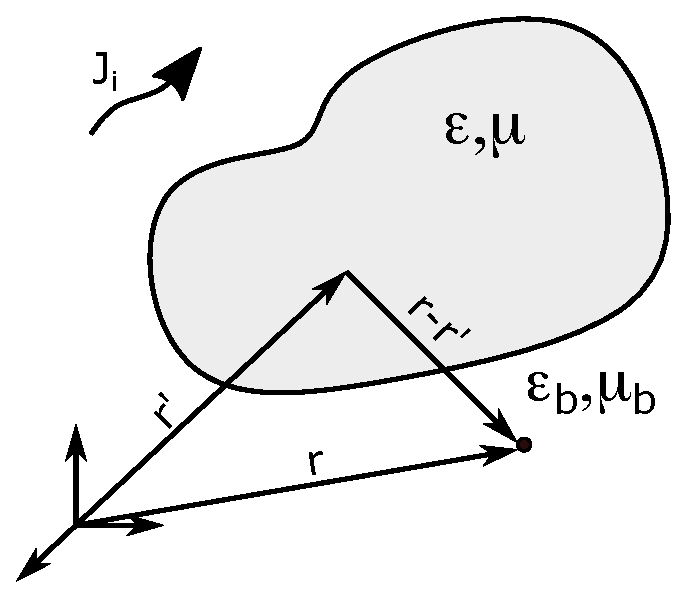
\includegraphics[width=0.5\textwidth]{./figuras/scattering}
			\caption{General scattering problem.}
			\label{fig:2:scattering}
		\end{figure}

		Um exemplo de múltiplas figuras pode ser visto na \autoref{fig:3:lcurve}.
		\begin{figure}[!htb]
			\centering
			\subfloat[]{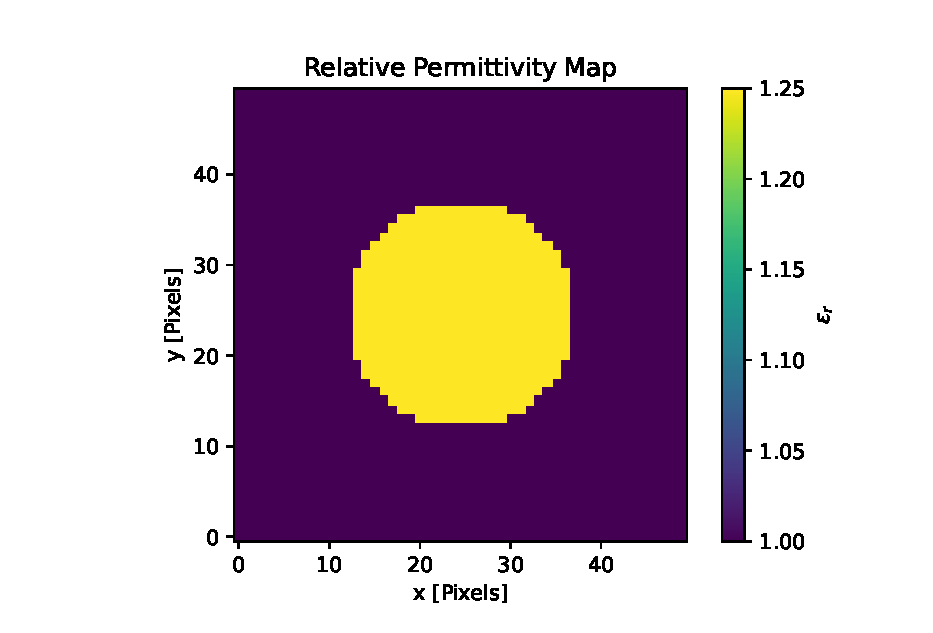
\includegraphics[width=.5\textwidth]{figuras/lcurve_input}}
			\subfloat[]{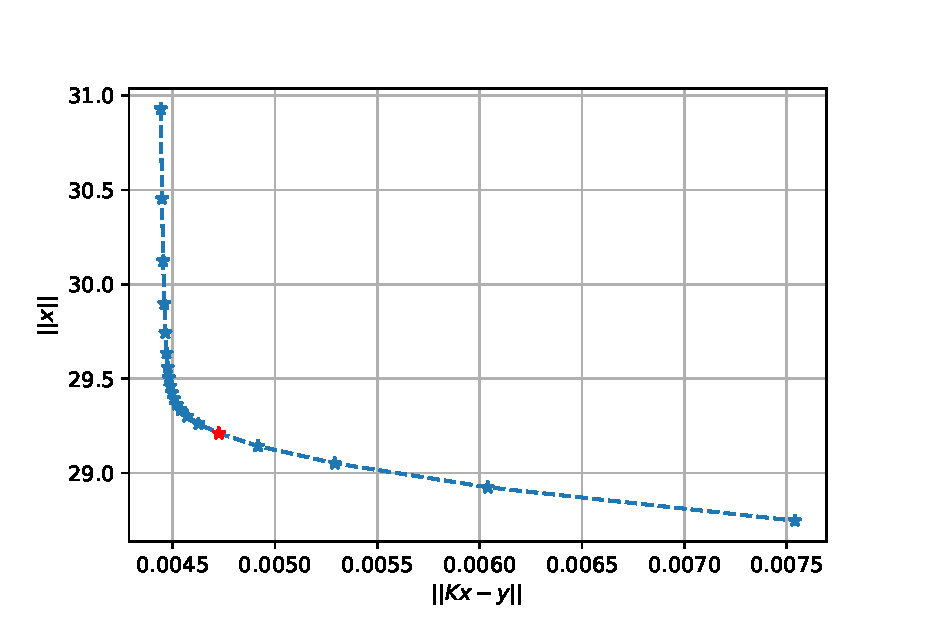
\includegraphics[width=.5\textwidth]{figuras/lcurve}} \\
			\subfloat[]{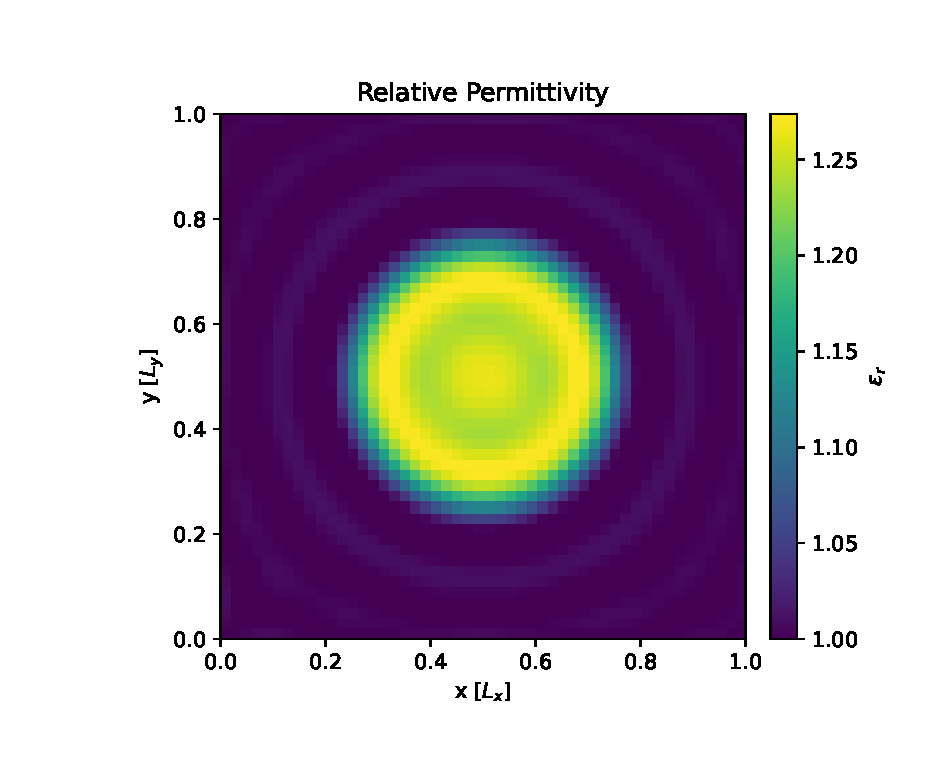
\includegraphics[width=.5\textwidth]{figuras/lcurve_result}}
			\caption[Exemplo de aplicação do Método da Curva-L.]{Example of applying the L-curve Method to a linear problem where it presupposes knowledge of the total field. (a) A simple instance of a contrast dielectric circle $\chi=0.25$ and radius $0.8\lambda_b$. Respecting the degrees of freedom, the scattered field was sampled in 45 positions for 45 incidence angles at a distance of $10\lambda_b$ from the center of the image. (b) L-curve considering 20 values of $\alpha_T$ in a range of $10^{-5}$ a $10^{-2}$. The red dot represents the solution with the shortest normalized distance to the origin. Its $\alpha_T$ value is approximately $2.3357 \times10^{-3}$. (c) Reconstruction of the image using the $\alpha_T$ value from the red dot. No inverse crime was committed since the data were obtained from the analytical solution.}
			\label{fig:3:lcurve}
		\end{figure}


		Um outro exemplode múltiplas figuras pode ser visto na \autoref{fig:proposed-methodology:surrogate:optimization:objfun}.
		\begin{figure}[!h]
			\centering
			\subfloat[]{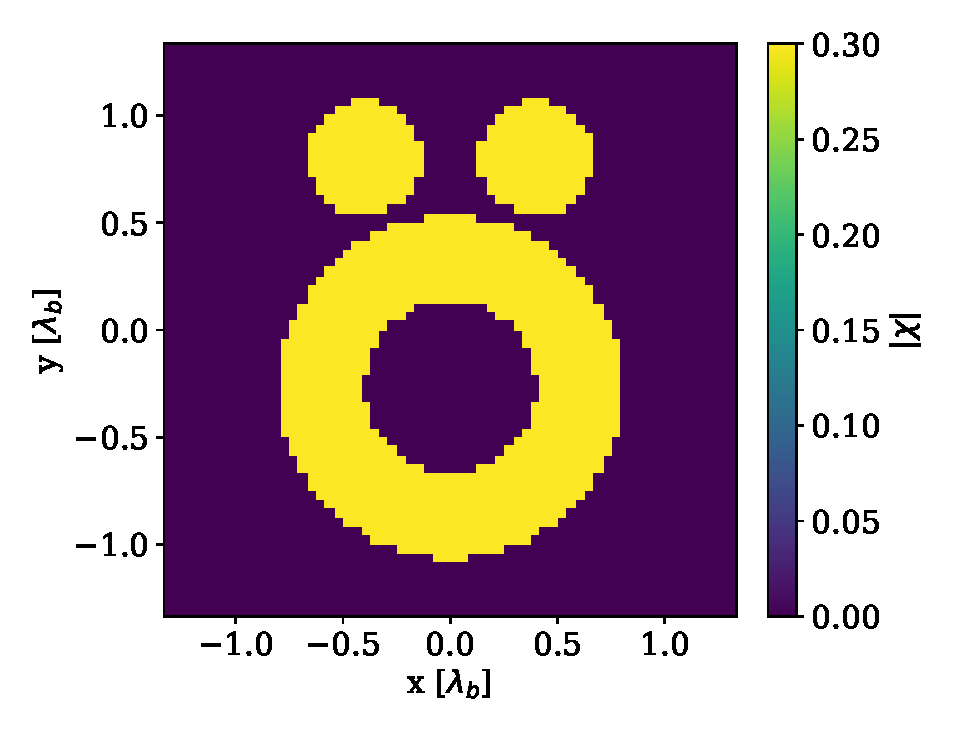
\includegraphics[width=.4\textwidth]{./figuras/objfun_groundtruth}\label{fig:proposed-methodology:surrogate:optimization:objfun:groundtruth}} \hspace{.05\textwidth}
			\subfloat[]{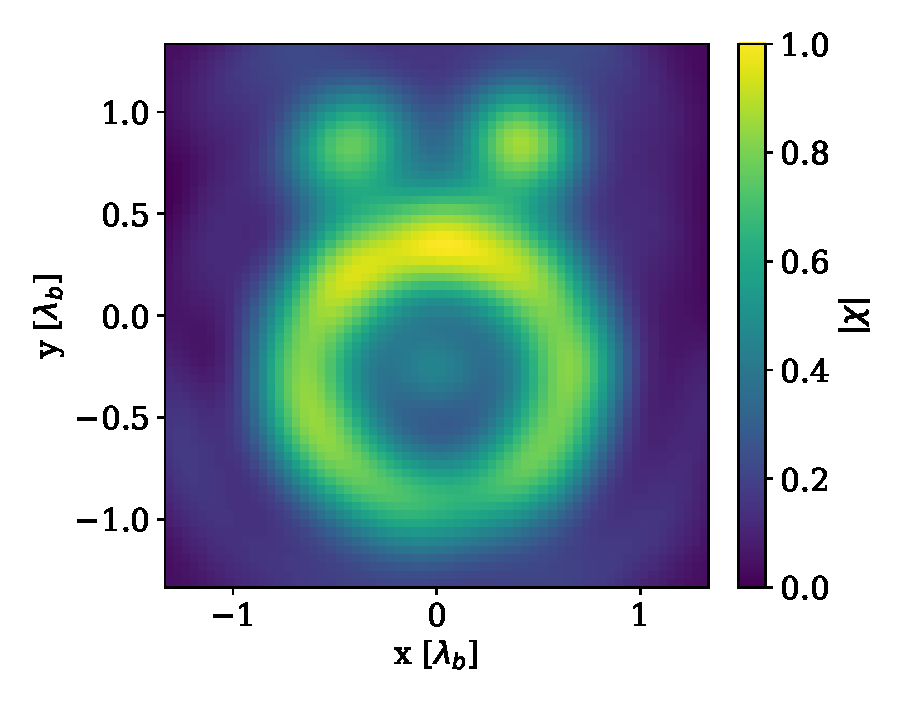
\includegraphics[width=.4\textwidth]{./figuras/objfun_qualitative}\label{fig:proposed-methodology:surrogate:optimization:objfun:qualitative}} \\
			\subfloat[]{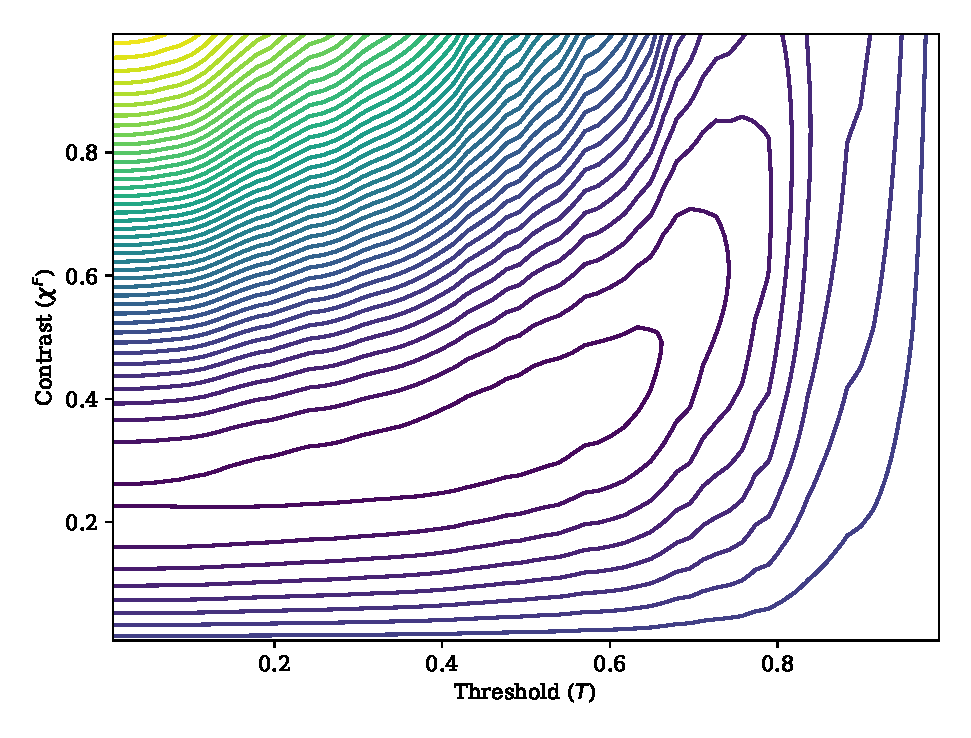
\includegraphics[width=.4\textwidth]{./figuras/objfun_surface}\label{fig:proposed-methodology:surrogate:optimization:objfun:surface}} \hspace{.05\textwidth}
			\subfloat[]{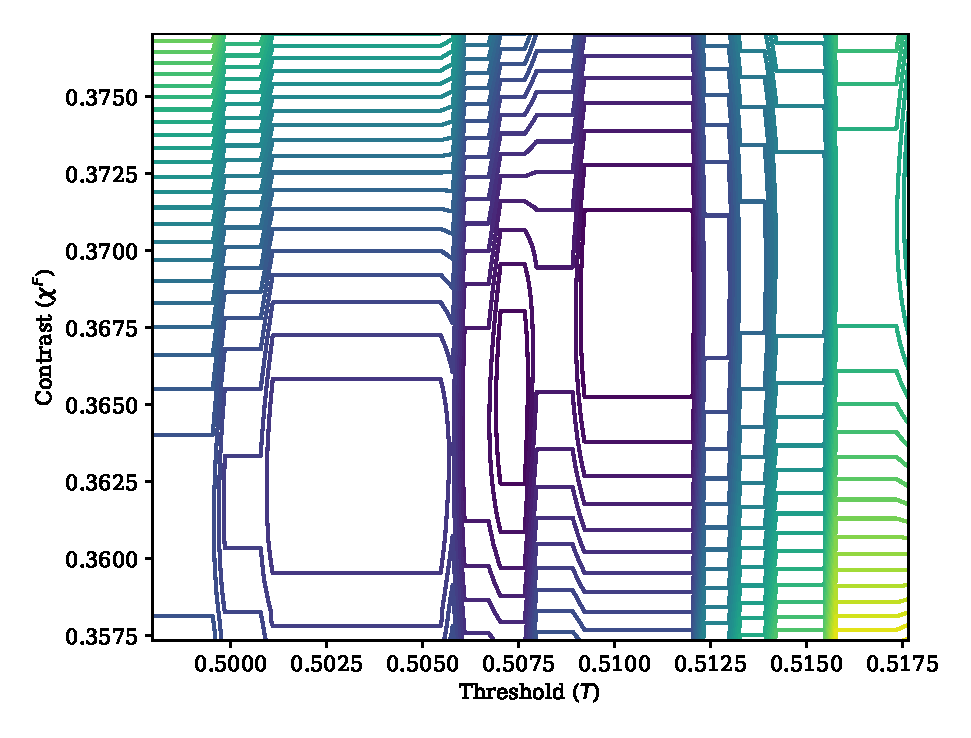
\includegraphics[width=.4\textwidth]{./figuras/objfun_nearoptimum}\label{fig:proposed-methodology:surrogate:optimization:objfun:nearoptimum}}
			\caption[Example of an objective function resulting from the transformation of the inversion problem into a two-dimensional optimization one.]{Example of an objective function resulting from the transformation of the inversion problem into a two-dimensional optimization one: (a) the ground-truth image; (b) the image obtained by OSM; (c) the surface obtained by the transformation of the inversion problem into a two-dimensional optimization one; and (d) a zoom over the region close to the optimum.}
			\label{fig:proposed-methodology:surrogate:optimization:objfun}
		\end{figure}

		Exemplo para inserir duas figuras horizontais \ref{fig:results:casestudy:austria:boxplot:zeta_eoe}:
		\begin{figure}
			\centering
			\subfloat[]{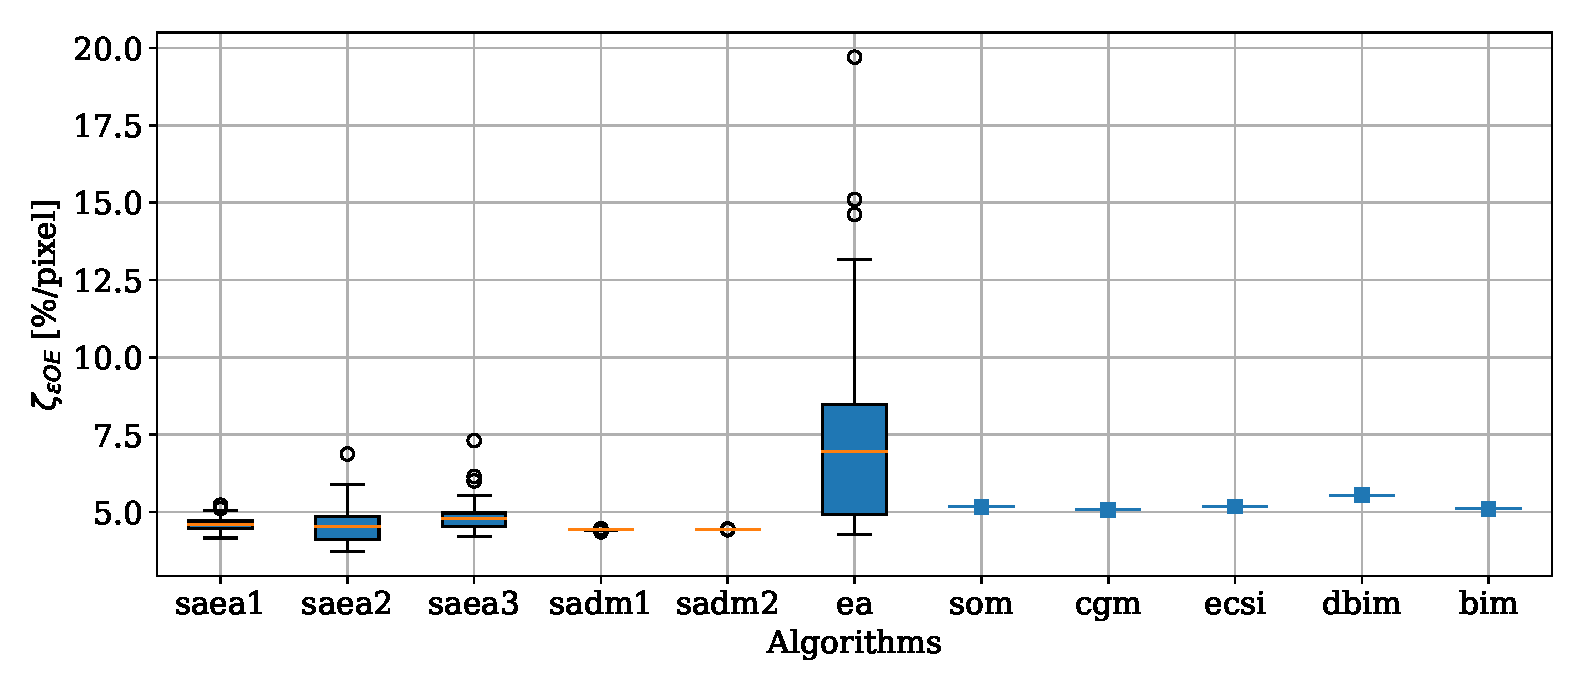
\includegraphics[width=.9\textwidth]{./figuras/casestudy/austria/boxplot_zeta_eoe_ea}\label{fig:results:casestudy:austria:boxplot:zeta_eoe:withea}} \\
			\subfloat[]{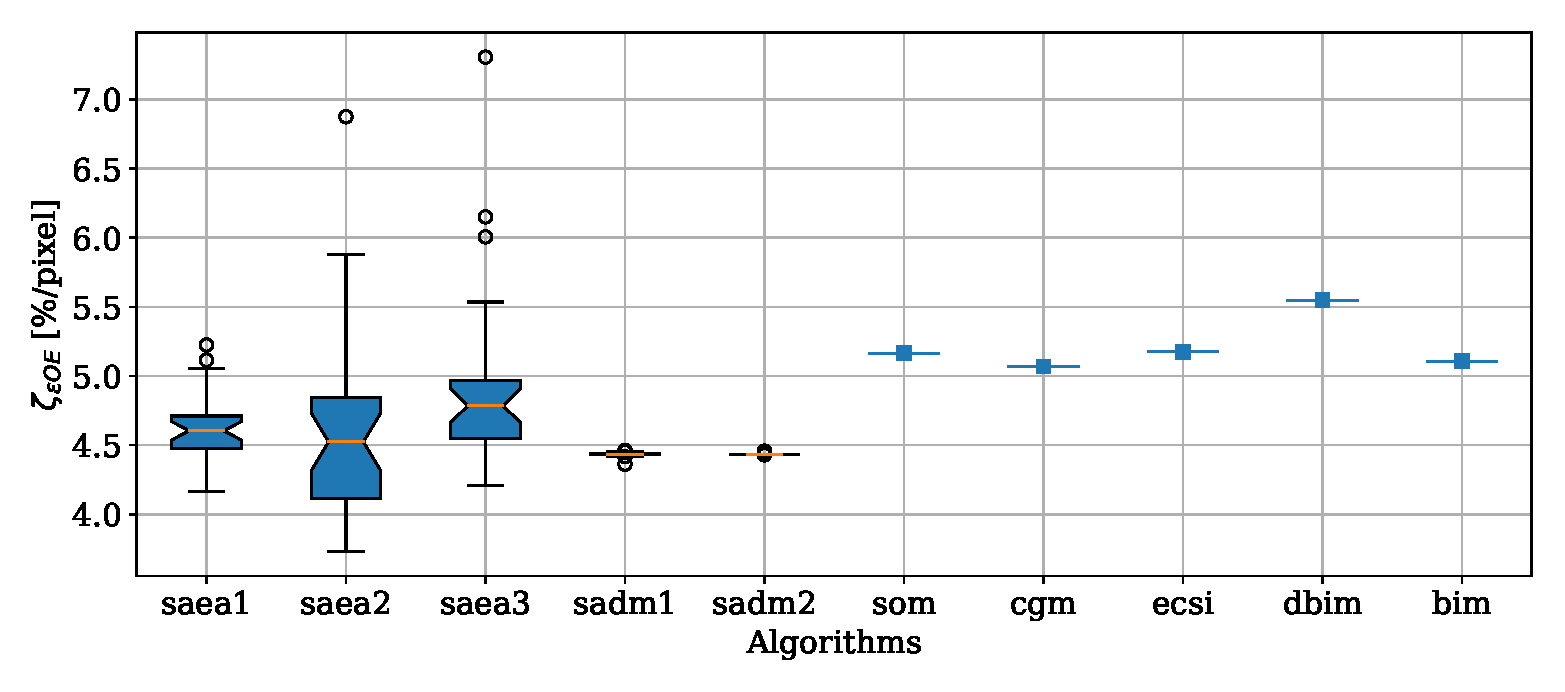
\includegraphics[width=.9\textwidth]{./figuras/casestudy/austria/boxplot_zeta_eoe}\label{fig:results:casestudy:austria:boxplot:zeta_eoe:noea}}
			\caption[Performance of $\zeta_{\epsilon OE}$ indicator for various algorithms in the Austria profile.]{Performance of $\zeta_{\epsilon OE}$ indicator for various algorithms in the Austria profile. (a) Boxplots show quartiles of 30 executions for stochastic algorithms, and the solid line represents the deterministic algorithms. (b) Exclusion of the EA algorithm for better visualization of differences among algorithms.}
			\label{fig:results:casestudy:austria:boxplot:zeta_eoe}
		\end{figure}
	
	\chapter{Como inserir tabelas}

		\renewcommand{\arraystretch}{1.3}

		Um exemplo de tabela simples é a \ref{tab:results:casestudy:austria:configuration}.
		\begin{table}[!h]
			\centering
			\caption[Parameters for Austria profile case study.]{Parameters for problem specification of Austria profile case study.}
			\rowcolors{1}{gray2}{gray1}
			\begin{tabular}{cccccc}
				$N_M$ & $N_S$ & $R_O$ & $f$ & $L_X$, $L_Y$ & $\epsilon_{rb}$ \\
				32 & 16 & 6 [m] & 400 [MHz] & 2 [m] & 1
			\end{tabular}
			\label{tab:results:casestudy:austria:configuration}
		\end{table}

		Um exemplo de tabela simples pode ser visto em \ref{tab:methods:conclusion}. Você pode referenciar tabelas da mesma forma que você referencia figuras. Por exemplo, você pode escrever: ``...como mostrado na \autoref{tab:methods:conclusion}, ...''.

		\begin{table}[]
			\setstretch{1.5}
			\caption{Classification of methods by their properties.}
			\label{tab:methods:conclusion}
			\begin{tabular}{clm{2cm}m{2cm}m{6cm}}
				\hline
				Classes & \multicolumn{4}{c}{Methods} \\ \hline
				\multirow{2}{*}{Qualitative} & \multicolumn{4}{l}{Linear Sampling Method} \\
				& \multicolumn{4}{l}{Orthogonality Sampling Method} \\ \hline
				\multirow{26}{*}{Quantitative} & \multirow{15}{*}{Deterministic} & \multirow{4}{*}{Linear} & \multicolumn{2}{l}{Born Approximation} \\
				&  &  & \multicolumn{2}{l}{Rytov Approximation} \\
				&  &  & \multicolumn{2}{l}{Back-Propagation Method} \\
				&  &  & \multicolumn{2}{l}{Dominant Current Scheme} \\ \cline{3-5} 
				&  & \multirow{11}{*}{Nonlinear} & \multirow{4}{*}{\makecell[l]{Forward\\and\\inverse\\subproblems}} & Born Iterative Method \\
				&  &  &  & Distorted Born Iterative Method \\
				&  &  &  & Variational Born Iterative Method \\
				&  &  &  & Level-Set Method \\ \cline{4-5} 
				&  &  & \multirow{3}{*}{\makecell[l]{Gradient-\\based}} & Conjugated-Gradient Method \\
				&  &  &  & Contrast Source Inversion \\
				&  &  &  & Subspace-based Optimization Method \\ \cline{4-5} 
				&  &  & \multirow{4}{*}{Other} & Compressive Sensing \\
				&  &  &  & Regularization on Lp Banach Spaces \\
				&  &  &  & Virtual Experiments \\
				&  &  &  & Deep learning methods \\ \cline{2-5} 
				& \multirow{11}{*}{Stochatisc} & Components & \multicolumn{2}{l}{Types} \\ \cline{3-5} 
				&  & \multirow{3}{*}{\makecell[l]{Representa-\\tion}} & \multicolumn{2}{l}{Known geometries} \\
				&  &  & \multicolumn{2}{l}{Contours} \\
				&  &  & \multicolumn{2}{l}{Pixel-based} \\ \cline{3-5} 
				&  & \multirow{2}{*}{\makecell[l]{Objective\\function}} & \multicolumn{2}{l}{Data equation residual} \\
				&  &  & \multicolumn{2}{l}{Data and state equation residual} \\ \cline{3-5} 
				&  & \multirow{3}{*}{Mechanism} & \multicolumn{2}{l}{GA} \\
				&  &  & \multicolumn{2}{l}{DE} \\
				&  &  & \multicolumn{2}{l}{PSO} \\ \cline{3-5} 
				&  & \multirow{2}{*}{\makecell[l]{Population\\Initialization}} & \multicolumn{2}{l}{Random} \\
				&  &  & \multicolumn{2}{l}{Born Approximation} \\\hline
			\end{tabular}
		\end{table}

		Exemplo de tabelas em landscape:

		\begin{landscape}
			\begin{table}[]
				 \footnotesize
				\centering
				\caption[P-values for posthoc multiple pairwise comparisons considering the $\zeta_{\epsilon OE}$ indicator.]{P-values for posthoc multiple pairwise comparisons considering the $\zeta_{\epsilon OE}$ indicator, with the compatible statistical test for each test set. The significance level has been corrected using the Bonferroni method, resulting in 0.0083. Detected differences are indicated in bold format. Confidence intervals are compute for means when Paired T-Test are evaluated and for medians when the Wilcoxon Signed-Rank Test is evaluated.}
				% \rowcolors{4}{gray2}{gray1}
				\begin{tabular}{ccccccccc}
					\multirow{2}{*}{Pairs} & \multicolumn{2}{c}{\begin{tabular}[c]{@{}c@{}}$\chi=0.5$\\ Wilcoxon\\ Signed-Rank test\end{tabular}} & \multicolumn{2}{c}{\begin{tabular}[c]{@{}c@{}}$\chi=1$\\ Paired T-Test\end{tabular}} & \multicolumn{2}{c}{\begin{tabular}[c]{@{}c@{}}$\chi=2$\\ Wilcoxon\\ Signed-Rank test\end{tabular}} & \multicolumn{2}{c}{\begin{tabular}[c]{@{}c@{}}$\chi=3$\\ Wilcoxon\\ Signed-Rank test\end{tabular}} \\ \cmidrule(rl){2-3} \cmidrule(rl){4-5} \cmidrule(rl){6-7} \cmidrule(rl){8-9} % \cline{2-9} 
					& p-value & Confi. In. & p-value & Confi. In. & p-value & Confi. In. & p-value & Confi. In. \\ \hline \rowcolor{gray1}
					SAEA1-SAEA2 & 0.2988 & (-0.031, 0.034) & $\boldsymbol{<}$\textbf{0.0001}  & (0.322, 0.895) & $\boldsymbol{<}$\textbf{0.0001} & (0.675, 1.576) & $\boldsymbol{<}$\textbf{0.0001} & (0.4, 1.484) \\\rowcolor{gray2}
					SAEA1-SAEA3 & 0.1706 & (0.012, 0.124) & $\boldsymbol{<}$\textbf{0.0001}  & (-2.5, -1.33) & $\boldsymbol{<}$\textbf{0.0001} & (-2.165, -0.916) & $\boldsymbol{<}$\textbf{0.0001} & (-2.574, -1.019) \\\rowcolor{gray1}
					SAEA1-SADM2 & 0.0577 & (-0.089, 0.002) & \textbf{0.003} & (-1.99, -0.132) &  0.6702  & (-0.804, 0.842) & 0.2054  & (-1.35, 0.862) \\\rowcolor{gray2}
					SAEA2-SAEA3 & 0.2988 & (-0.017, 0.148) & $\boldsymbol{<}$\textbf{0.0001} & (-3.18, -1.87) & $\boldsymbol{<}$\textbf{0.0001} & (-4.152, -2.3) & $\boldsymbol{<}$\textbf{0.0001} & (-4.301, -2.237) \\\rowcolor{gray1}
					SAEA2-SADM2 & 0.0164 & (-0.109, -0.009) & $\boldsymbol{<}$\textbf{0.0001} & (-2.71, -0.634) & \textbf{0.0008} & (-1.542, -0.063) & \textbf{0.0015} & (-2.494, 0.137) \\\rowcolor{gray2}
					SAEA3-SADM2 & 0.1347 & (-0.21, -0.023) & 0.023 & (-0.153, 1.86) & 0.0113 & (0.912, 3.128) & 0.1642 & (-0.886, 2.103)
				\end{tabular}
				\label{tab:results:benchmark:zetaeoe:pvalues}
			\end{table}
		
			\begin{table}[]
				\centering
				\footnotesize
				\caption[P-values for posthoc multiple pairwise comparisons considering the $\zeta_{S}$ indicator.]{P-values for posthoc multiple pairwise comparisons obtained by Wilcoxon Signed-Rank tests considering the $\zeta_S$ indicator. The significance level has been corrected using the Bonferroni method, resulting in 0.0083. Detected differences are indicated in bold format. The confidence interval for medians is also presented.}
				% \rowcolors{3}{gray2}{gray1}
				\begin{tabular}{ccccccccccc}
					\multirow{2}{*}{Pairs} & \multicolumn{2}{c}{\begin{tabular}[c]{@{}c@{}}$\chi=0.5$\end{tabular}} & \multicolumn{2}{c}{\begin{tabular}[c]{@{}c@{}}$\chi=1$\end{tabular}} & \multicolumn{2}{c}{\begin{tabular}[c]{@{}c@{}}$\chi=2$\end{tabular}} & \multicolumn{2}{c}{\begin{tabular}[c]{@{}c@{}}$\chi=3$\end{tabular}} & \multicolumn{2}{c}{\begin{tabular}[c]{@{}c@{}}$\chi=4$\end{tabular}} \\ \cmidrule(rl){2-3} \cmidrule(rl){4-5} \cmidrule(rl){6-7} \cmidrule(rl){8-9} \cmidrule(rl){10-11} % \cline{2-11} 
					& p-value & Confi. In. & p-value & Confi. In. & p-value & Confi. In. & p-value & Confi. In. & p-value & Confi. In. \\ \hline \rowcolor{gray1}
					SAEA1-SAEA2             & $\boldsymbol{<}$\textbf{0.0001} & (0.34, 0.92)   & $\boldsymbol{<}$\textbf{0.0001} & (0.49, 1.09)     & $\boldsymbol{<}$\textbf{0.0001} & (1.02, 2.04)   & \textbf{0.0002}        & (0.67, 2.01)   & 0.0145                 &  (0.2, 2)                                      \\\rowcolor{gray2}
					SAEA1-SAEA3             & \textbf{0.0002}        & (-1.32, -0.49) & $\boldsymbol{<}$\textbf{0.0001} & (-5.38, -3.52) & $\boldsymbol{<}$\textbf{0.0001} & (-2.46, -1.34) & $\boldsymbol{<}$\textbf{0.0001} & (-3.16, -1.28)   & \textbf{0.0066} & (-3.08, -0.92)                                       \\\rowcolor{gray1}
					SAEA1-SADM2             & \textbf{0.0012}        & (0.02, 0.69)    & \textbf{0.0081}        & (-2.38, 0.37)   & 0.3931                      & (-0.85, 0.59) & 0.1706                     & (-1.72, 1.16)   & 0.9515                & (-1.70, 1.58)                                        \\\rowcolor{gray2}
					SAEA2-SAEA3             & $\boldsymbol{<}$\textbf{0.0001} & (-2.15, -0.97) & $\boldsymbol{<}$\textbf{0.0001} & (-5.80, -3.40) & $\boldsymbol{<}$\textbf{0.0001} & (-4.69, -1.97) & $\boldsymbol{<}$\textbf{0.0001} & (-5.73, -2.71) & \textbf{0.0028} &(-4.79, -1.37)                                        \\\rowcolor{gray1}
					SAEA2-SADM2             & 0.1996                     & (-0.20, 0.15)  & $\boldsymbol{<}$\textbf{0.0001} & (-2.64, -0.17)  & $\boldsymbol{<}$\textbf{0.0001} & (-2.70, -0.66) & \textbf{0.0007}       & (-3.61, 0.08)   & 0.1059             & (-2.17, 0.72)                                        \\\rowcolor{gray2}
					SAEA3-SADM2             & $\boldsymbol{<}$\textbf{0.0001} & (0.51, 1.82)    & \textbf{0.0081}        & (0.91, 3.32)     & 0.0087                       & (0.83, 2.88)   & 0.2801                    & (-0.62, 1.93)   & 0.1094             & (0.67, 4.32)                                                         
				\end{tabular}
				\label{tab:results:benchmark:zetas:pvalues}
			\end{table}
		\end{landscape}
	
	\chapter{Como inserir algoritmos}

		Um exemplo de algoritmo é o seguinte:
		\begin{algorithm}[!htb]
			\caption{Distorted Born Iterative Method.}
			\label{alg:dbim}
			\KwIn{$\mathbf{\bar{E}^s}$, $\mathbf{\bar{G}^{2D}}$, $\mathbf{\bar{G}^S}$}
			\KwOut{$\boldsymbol{\bar{\chi}}$, $\mathbf{\bar{E}}$}
			Compute an initial guess $\boldsymbol{\bar{\chi}^0}$ based on available information \\
			$t\leftarrow0$ \\
			\While{some criterion is not reached} {
				Solve $\left(\mathbf{\bar{I}} - \mathbf{\bar{G}^S}\boldsymbol{\bar{\chi}}^t\right)\mathbf{\bar{G}}^{\mathbf{in},t} = \mathbf{\bar{G}^{2D}}$ for $\mathbf{\bar{G}}^{\mathbf{in},t}$ \\
				Solve the direct problem for $\mathbf{\bar{E}}^t$ and $\mathbf{\bar{E}}^{\mathbf{s},t}$ \\
				$\Delta\mathbf{\bar{E}^s} = \mathbf{\bar{E}}^s - \mathbf{\bar{E}}^{\mathbf{s},t}$ \\
				Solve the inverse linear problem $\Delta\mathbf{\bar{E}^s} = \mathbf{\bar{G}}^{\mathbf{in},t}\Delta\boldsymbol{\bar{\chi}}\mathbf{\bar{E}}^t$ for $\Delta\boldsymbol{\bar{\chi}}$\\
				$\boldsymbol{\bar{\chi}}^t \leftarrow \boldsymbol{\bar{\chi}}^{t-1} + \Delta\boldsymbol{\bar{\chi}}^t$ \\
				$t\leftarrow t+1$\\
			}
		\end{algorithm}
	
	\chapter{Como inserir definições e outras coisas especiais}

		Um exemplo de definição:
		\begin{definition}\label{def:3:projection}
			Projection Operator\\
			Let $X$ be a normed space over the field $\mathbb{K}=\mathbb{R}$ or $\mathbb{K}=\mathbb{C}$. Let $U\subset X$ be a closed subspace. A linear bounded operator $\mathcal{P} : X\rightarrow X$ is called a projection operator on $U$ if
			\begin{itemize}
				\item $\mathcal{P}\{x\} \in U, ~\forall x\in X$ and
				\item $\mathcal{P}\{x\} = x,~ \forall x\in U$.
			\end{itemize}
		\end{definition}

		Um exemplo de teorema:
		\begin{theorem}\label{the:app:functional:1}
			Let $X$ be a pre-Hilbert space. The mapping $||\cdot|| : X\rightarrow\mathbb{R}$ defined by $$||x||\coloneqq\sqrt{\langle x,x\rangle},~x\in X$$ is a norm. Futhermore:
			\begin{enumerate}
				\item $|(x,y)|\le||x||||y||,~\forall x,y\in X$ (Cauchy-Schwarz inequality);
				\item $||x\pm y||^2 = ||x||^2+||y||^2\pm 2\mathfrak{Re}\{\langle x,y\rangle\}\forall x,y\in X$ (binomial formula);
				\item  $||x+y||^2 + ||x-y||^2 = 2||x||^2+2||y||^2\forall x,y\in X$.
			\end{enumerate}
		\end{theorem}

		Um exemplo de código em Python:

		\begin{lstlisting}[language=Python]
# Evaluate contourns
co = measure.find_contours(original, 1.0, fully_connected='high')
cr = measure.find_contours(recovered, threshold)
			
# Converting scale of recovered contourn
for i in range(len(cr)):
    cr[i][:, 1] = original.shape[1]*cr[i][:, 1]/recovered.shape[1]
    cr[i][:, 0] = original.shape[0]*cr[i][:, 0]/recovered.shape[0]
			
# Thresholding
masko = np.zeros(original.shape, dtype=bool)
maskr = np.zeros(recovered.shape, dtype=bool)
masko[original > 1] = True
maskr[recovered >= threshold] = True
			
# Evaluate centers
xo, yo = np.meshgrid(np.arange(0, original.shape[1]),
                     np.arange(0, original.shape[0]))
xr, yr = np.meshgrid(np.linspace(0, original.shape[1]-1, 
                                 recovered.shape[1]),
                     np.linspace(0, original.shape[0]-1,
                                 recovered.shape[0]))
xco = np.sum(masko*xo)/np.sum(masko)
yco = np.sum(masko*yo)/np.sum(masko)
xcr = np.sum(maskr*xr)/np.sum(maskr)
ycr = np.sum(maskr*yr)/np.sum(maskr)
			
# Centralization
for i in range(len(co)):
    co[i][:, 0] = co[i][:, 0]-yco+original.shape[0]/2
    co[i][:, 1] = co[i][:, 1]-xco+original.shape[1]/2
			
# Centralization
for i in range(len(cr)):
    cr[i][:, 0] = cr[i][:, 0]-ycr+original.shape[0]/2
    cr[i][:, 1] = cr[i][:, 1]-xcr+original.shape[1]/2
			
# Verify points
masko = np.zeros(original.shape, dtype=bool)
counter = np.zeros(original.shape)
for i in range(len(co)):
    maskt = measure.grid_points_in_poly(original.shape, co[i])
    counter[maskt] += 1
    masko[np.mod(counter, 2) == 1] = True
			
# Verify points
maskr = np.zeros(original.shape, dtype=bool)
counter = np.zeros(original.shape)
for i in range(len(cr)):
    maskt = measure.grid_points_in_poly(original.shape, cr[i])
    counter[maskt] += 1
    maskr[np.mod(counter, 2) == 1] = True
			
# Xor operation
diff = np.logical_xor(masko, maskr)
			
# Area of the difference
zeta_s = np.sum(diff)/np.sum(masko)*100
			
# Figure
fig, axis = plt.subplots(ncols=3, figsize=[3*6.4,4.8])
fig.subplots_adjust(wspace=.5)
axis[0].imshow(masko, origin='lower')
axis[0].set_title('Original')
axis[1].imshow(maskr, origin='lower')
axis[1].set_title('Recovered')
axis[2].imshow(diff, origin='lower')
axis[2].set_title('Difference')
			
plt.show()
\end{lstlisting}




\end{document}
